\documentclass[12pt]{article}

\usepackage[left=2.3cm, right=2.3cm, top=1.7cm, bottom=1.7cm]{geometry}
\usepackage{amsmath}

\usepackage{hyperref}
\hypersetup{
    colorlinks=true,      % false: boxed links; true: colored links
    linkcolor=black,      % color of internal links (change box color with linkbordercolor)
    urlcolor=black        % color of external links
}
\usepackage{tikz}
\usetikzlibrary{positioning}


\usepackage{Sweave}
\begin{document}
\input{worksheet-concordance}

% \section*{Name:} \vspace{0.4cm}

\begin{center}
{\Huge Quadratics}
\end{center}

The first two sections of this document contain mostly information, they can be abit dense so feel free to skip ahead to the sections with more excercises and then refer back to these sections later for information as you need it:
\begin{itemize}
  \item \textbf{Introduction}: although we will be focused on learning about quadratics, in this section quadratics are placed into the broader picture of functions and polynomials. The main purpose of this section beyond putting quadratics into a broader context is to provide an introduction to some of the language, terminology, and notation around functions and polynomials.
  \item \textbf{Quadratics}: here we get into the main learning intentions, and summarising the activities you will be doing.
\end{itemize}

The remaining sections each focus on a key concept or skill, mostly consisting of exercises for practice. You can move through these at your own pace, but make sure you do at least a couple of excersises from each section.
\begin{itemize}
  \item \textbf{Expanding Brackets}: this should be revision but is important to practice,
  \item \textbf{Factorising}: is the reverse of expanding brackets, essentially, but is important for dealing with more complex functions.
  \item \textbf{Special Cases}: introduces the special cases ``difference of two squares'' and ``perfect squares''.
  \item \textbf{Complete the Square}: is a key skill that uses expanding brackets, factorising, and ``perfect squares'', so make sure you have practiced those things before you attempt this section.
\end{itemize}


\section*{Introduction}

A \textbf{function} is a thing into which you can input a number, and that will output a number in response. This can be schematically represented as:

\begin{center}
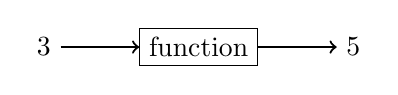
\begin{tikzpicture}

\node (a) at (0,0) {3};
\node[right = 1cm of a, rectangle, draw] (b) {function};
\node[right = 1cm of b] (c) {5};
\draw[->, thick] (a) -- (b);
\draw[->, thick] (b) -- (c);

\end{tikzpicture}
\end{center}

Often, we label the input $x$ and the output $y$, as we will typically graph the inputs horizontally and the outputs vertically. 

If we name our function $f$, then we can represent this as:

\begin{center}
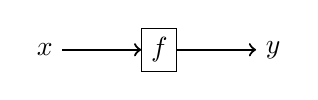
\begin{tikzpicture}

\node (a) at (0,0) {$x$};
\node[right = 1cm of a, rectangle, draw] (b) {$f$};
\node[right = 1cm of b] (c) {$y$};
\draw[->, thick] (a) -- (b);
\draw[->, thick] (b) -- (c);

\end{tikzpicture}
\end{center}
and understand this as ``$x$ goes into $f$, and $y$ comes out''.

Importantly, this is often written as 
\begin{equation*}
f(x) = y
\end{equation*}
with the input to the function ($x$ in this case) in brackets infront of the name of the function ($f$ in this case), which all evaluates (equals) the output ($y$ in this case). 

The above example with input $3$ and output $5$ could be many different functions. For example:

\begin{align*}
\text{if} \quad   f(x)  &= 2x - 1   & \text{if} \quad   f(x)  &= 3x^2 -5x - 7   \\
\text{then} \quad f(3)  &= 2(3) - 1 & \text{then} \quad f(3)  &= 3(3)^2 -5(3) - 7 \\
                        &= 6 - 1    &                         &= 27 - 15 - 7 \\
                        &= 5        &                         &= 5 \\
\end{align*}

\textbf{Polynomials} are functions that produce an output by raising the input to \emph{whole number} powers and then multiply and add the results by other numbers called \textbf{coefficients}. The following are all examples of \textbf{polynomial functions}:

\begin{itemize}
  \item $f(x) = x^2 + x + 1$,
  \item $f(x) = x^5 + 3x^4 - 7x^3 + 4x^2 - 5x + 2$,
  \item $f(x) = 2x^3 - 1$,
  \item $f(x) = x^2$,
  \item $f(x) = 7$. 
\end{itemize}

\vspace{0.2cm}\fbox{\begin{minipage}{\linewidth}Extension question: Why does $f(x) = 7$ count as a polynomial function? How is it using a whole number power of the input?\end{minipage}}\vspace{0.2cm}

\textbf{Quadratics} are polynomials whose highest power of the input (that is not multiplied by zero) is $2$. So for example, the folling are examples of quadratics:

\begin{itemize}
  \item $f(x) = x^2 + x + 1$,
  \item $f(x) = x^2$,
  \item $f(x) = 3x^2 + 7$.
\end{itemize}

However a function like $f(x) = 0x^2 + x + 3 = x + 3$ would not be called a quadratic.

Another name for quadratics is ``polynomials of order $2$'' because they are polynomials whose highest power is $2$. In this sense there are also polynomails of order $3$ (which are called cubics), of order 4 (which are called quartics), and of every other order. 

\vspace{0.2cm}\fbox{\begin{minipage}{\linewidth}Extension question: What do you think polynomials of order 5 should be called? \end{minipage}}\vspace{0.2cm}

% Finally, we use the word ``\textbf{coefficient}'' to refer to the numbers multiplied by each term in a polynomial. So for example, the $x^2$ term has coefficient $3$ in the quadratic $f(x) = 3x^2 + 5x - 4$. 
% 
% Bonus question: In the quadratic above, $f(x) = 3x^2 + 5x - 4$, $4$ is also considered a coefficient, but what power of $x$ is it multiplied by?

\section*{Quadratics}

Quadratics (or polynomials of order $2$) are important, as they form the foundation of all polynomial functions.
There are three ways we can write quadratics, what we will be learning in this section is:
\begin{itemize}
  \item How to convert between the different forms of a quadratic.
  \item How to use (interpret) each form in terms of being able to determine facts about the graph of the function.
\end{itemize}

To understand how to intpret each of the forms, take a look at the corresponding GeoGebra activities linked below and see if you can determine the effect the various sliders have on the graph of the function in each case.

The three forms of a quadratic are:
\begin{itemize}
  \item \textbf{General Form}: written $f(x) = ax^2 + bx + c$. See the GeoGebra activity: \url{https://ggbm.at/swgr9vr3}, 
  \item \textbf{Vertex Form}: written $f(x) = a(x - b)^2 + c$. See the GeoGebra activity: \url{https://ggbm.at/hezgak8s}, and
  \item \textbf{Factorised Form}: written $f(x) = a(x - b)(x - c)$. See the GeoGebra activity: \url{https://ggbm.at/f8wyvqad}.
\end{itemize}

Some important notes:
\begin{itemize}
  \item Every quadratic can be written in general and vertex forms, but only some quadratics can be written in factorised form.
  \item A quadratic written in either vertex or factorised form can be re-written in general form simply by \textbf{expanding brackets}.
  \item A quadratic written in general form can be converted to factorised form by a process called \textbf{factorisation}, or to vertex form by a process called \textbf{completing the square}.
\end{itemize}

The remaining sections will involve learning, practicing, and developing an understanding of the skills surrounding these three processes:
\begin{itemize}
  \item \textbf{Expanding brackets},
  \item \textbf{Factorisation}, and
  \item \textbf{Completing the square},
\end{itemize}
as these skills are important not only for manipulating and understanding quadratics, but also for higher order polynomials and other functions as well. They form a core set of skills that will be useful throughout every mathematics topic.


\pagebreak
\section*{Expanding Brackets}


Simple brackets can be expanded using the \textbf{distributive law}, here are two examples of what that looks like:

\begin{align*}
2(x + 3)  &= 2(x) + 2(3)  & x(x - 3)  &= x(x) + x(-3) \\
          &= 2x + 6       &           &= x^2 - 3x \\ 
\end{align*}

But in more complex examples such as for example $(x+2)(x+5)$, this is often taught in terms of FOIL (Firsts Outers Inners Lasts), which would allow you to expand $(x+2)(x+5)$ as follows:

\begin{align*}
(x+2)(x+5)  &= x(x) + x(5) + 2(x) + 2(5) \\
            &= x^2 + 5x + 2x + 10 \\
            &= x^2 + 7x + 10 \\
\end{align*}

This works fine, but another approach to doing the same thing (that also happens to generalise better) is to simply use the distributive law twice, which looks like: 

\begin{align*}
(x+2)(x+5)  &= x(x+5) + 2(x+5) \\
            &= x(x) + x(5) + 2(x) + 2(5) \\
            &= x^2 + 5x + 2x + 10 \\
            &= x^2 + 7x + 10 \\
\end{align*}

Which of course gives you the same answer. This is infact where the FOIL shortcut comes from. In this context you can use whichever method is easier for you. 

Even if this seems straightforward to you, it is important to practice it as it is easy to make mistakes, particularly in more difficult examples which involve double-negatives, etc. So at least do each of the exercises in the lefthand most column.

\pagebreak
\subsection*{Exercises:}
Expand the brackets to write each of the following quadratics in general form. \\

\begin{center}
\begin{tabular}{rlrlrl}
(a) & $(x+1)(x+2)$ & (b) & $(x+3)(x+7)$ & (c) & $(x+10)(x+17)$ \\
(d) & $(x+3)(x-1)$ & (e) & $(x-5)(x+8)$ & (f) & $(x+2)(x-5)$ \\
(g) & $(x-1)(x-3)$ & (h) & $(x-6)(x-1)$ & (i) & $(x-3)(x-5)$ \\
(j) & $(-x+2)(x-5)$ & (k) & $(x+7)(-x-8)$ & (l) & $(-x+2)(x-5)$ \\
(m) & $(3-x)(x-3)$ & (n) & $(-8-x)(x-8)$ & (o) & $(-x+3)(5-x)$ \\
(p) & $(2-3x)(5x-4)$ & (q) & $(-7-x)(8x-2)$ & (r) & $(-2x+4)(1-7x)$ \\
(s) & $2(1-2x)(3x-1)$ & (t) & $5(-3-x)(x-2)$ & (u) & $4(-5x+1)(1-x)$ \\
(v) & $2(x-\frac{1}{2})(5-\frac{x}{2})$ & (w) & $3(\frac{-5}{9}-x)(x-{\frac{1}{3}})$ & (x) & $24(-x+3)(5-x)$ \\
\end{tabular}
\end{center}

Expand the brackets to write each of the following quadratics in general form. \\

\begin{center}
\begin{tabular}{rlrlrl}
(a) & $2(x-1)^2 - 3$ & (b) & $\frac{1}{2}(2x-5)^2 + \frac{5}{2}$ \\
\end{tabular}
\end{center}

\vspace{0.2cm}\fbox{\begin{minipage}{\linewidth}
Extension: Try expanding a cubic like $2(x-1)(x+1)(x-4)$
\end{minipage}}\vspace{0.2cm}


\pagebreak
\section*{Factorising}

Factorising a quadratic is essentially the opposite process to expanding brackets --- you add brackets, but this is much more difficult. A generally good process to follow is: 
\begin{enumerate}
  \item Factor out the coefficient of the $x^2$ term, so ``$a$'' in general form.
  \item List the factors of the remaining constant term (so ``$c$'' in general form) and sum each pair of factors. If the result of this sum is equal to the coefficient of the $x$ term (``$b$'' in general form), these factors can be used to factorise the quadratic.
  \item Use the factors identified to factorise the quadratic (see example below). Note that not all quadratics can be factorised, so if you summed each pair of factors and didn't get the coefficient of the $x$ term, it is possible that that quadratic can't be factorised.
  \item Expand the brackets again to check you get what you started with, ensuring that you haven't made any mistakes.
\end{enumerate}

\subsection*{Worked example:} 
Let's factorise $2x^2 + 12x - 54$.
\begin{enumerate}
  \item First, we factor out the coefficient of the $x^2$ term, in this case $2$. This will give us 
    \begin{equation*}
      2x^2 + 12x - 54 = 2(x^2 + 6x - 27)
    \end{equation*}

  \item Now we list the factors of the remaining constant term, in this case $-27$. Each pair of factors sum to $1 + (-27) = -26$, $(-1) + 27 = 26$, $3 + (-9) = -6$, and $(-3) + 9 = 6$. By matching these sums to the coefficient of $x$ (in this case $6$) we can see the factors we need are $-3$ and $9$. 
  
  \item So, we can factorise our quadratic as follows:
    \begin{align*}
      2x^2 + 12x - 54 &= 2(x^2 + 6x - 27) \\
                      &= 2(x+9)(x-3) \\
    \end{align*}
    Note how the $+9$ and the $-3$ are our factors.

  \item Finally, all we have to do is check we haven't made any mistakes. We can do this by expanding brackets again to check that we get back to where we started:
    \begin{align*}
      2(x+9)(x-3) &= 2(x(x-3) + 9(x-3)) \\
                  &= 2(x(x) + x(-3) + 9(x) + 9(-3)) \\
                  &= 2(x^2 - 3x + 9x -27) \\
                  &= 2(x^2 + 6x - 27) \\
                  &= 2(x^2) + 2(6x) + 2(-27) \\
                  &= 2x^2 + 12x -54 \\
    \end{align*}
  Which is what we started with, so we got it right! 
\end{enumerate}

Time for you to try it and practice with some exercises.

\pagebreak
\subsection*{Exercises:}
Write the following quadratics in factorised form. \\
\begin{center}
\begin{tabular}{rlrlrl}
(a) & $x^2 + 3x + 2$ & (b) & $x^2 + 4x + 3$ & (c) & $x^2 + 6x + 5$ \\
(d) & $x^2 + 6x + 8$ & (e) & $x^2 + 7x + 12$ & (f) & $x^2 + 8x + 12$ \\
(g) & $x^2 - 6x - 16$ & (h) & $x^2 + -10x + 16$ & (i) & $x^2 + 5x - 14$ \\
(j) & $2x^2 -20x + 18$ & (k) & $3x^2 + 9x + 6$ & (l) & $5x^2 + 50x + 45$ \\
\end{tabular}
\end{center}

\vspace{0.2cm}\fbox{\begin{minipage}{\linewidth}
Extension: Try factorising $5x^2 + 17x - 12$
\end{minipage}}\vspace{0.2cm}

\pagebreak
\section*{Special Cases}

This section covers two special kinds of quadratics. These special quadratics are useful to know about because they allow us to take shortcuts when expanding brackets and factorising.

\subsection*{Difference of Two Squares}

\textbf{Difference of Two Squares} is when a quadratic can be written as the difference of two squares: 
\begin{equation*}
x^2 - a^2.
\end{equation*}
For example let's consider $x^2 - 9 = x^2 - 3^2$. This can be factorised easily into  
\begin{equation*}
x^2 - 9 = x^2 - 3^2 = (x+3)(x-3). 
\end{equation*}
By expanding brackets we can both check the factorisation above is correct, and also gain some insight into why this works out so neatly:
\begin{align*}
(x+3)(x-3)  &= x(x-3) + 3(x-3) \\
            &= x(x) + x(-3) + 3(x) + 3(-3) \\
            &= x^2 -3x + 3x - 9 \\
            &= x^2 - 9 \\
\end{align*}
Note how the $-3x$ and $+3x$ terms cancel each other out. 

\textbf{Note:} If the $x^2$ term has a number multiplied by it you should factor that out first.



\subsection*{Perfect Squares}

\textbf{Perfect Squares} is when a quadratic can be written in the form: 
\begin{equation*}
(x + a)^2.
\end{equation*}
which if we expand the bracket gives us
\begin{equation*}
(x + a)(x + a) = x^2 + 2ax + a^2
\end{equation*}

To factorise a ``perfect squares'' quadratic, identify ``$a$'' in the above expression by halving the coefficient of $x$. So for example, to factorise $x^2 + 6x + 9$ take half $6$ (so, $3$), so we can write $x^2 + 6x + 9 = (x+3)^2$. As usual, we can check that this is correct by expanding the brackets.

\textbf{Note:} Also as usual, if the $x^2$ term has a number multiplied by it you should factor that out first.

\pagebreak
\subsection*{Exercises:}

Write the following quadratics in factorised form using what you know about ``Difference of two Squares''. \\
\begin{center}
\begin{tabular}{rlrlrl}
(a) & $x^2 - 25$ & (b) & $x^2 -81$ & (c) & $x^2 -144$ \\
(d) & $2x^2 - 72$ & (e) & $5x^2 - 80$ & (f) & $3x^2 -147$ \\
(g) & $2x^2 - \frac{1}{2}$ & (h) & $x^2 - \frac{4}{9}$ & (i) & $3x^2 - \frac{12}{25}$ \\
\end{tabular}
\end{center}

Write the following quadratics in factorised form using what you know about ``perfect squares''. \\
\begin{center}
\begin{tabular}{rlrlrl}
(a) & $x^2 + 4x + 4$ & (b) & $x^2 + 10x + 25 $ & (c) & $x^2 + 18 + 81$ \\
(d) & $x^2 -8x + 16$ & (e) & $x^2 - 12x + 36$ & (f) & $x^2 - 16x + 64$ \\
\end{tabular}
\end{center}

\vspace{0.2cm}\fbox{\begin{minipage}{\linewidth}
Extension: Try factorising $3x^2 - 3x + \frac{3}{4}$ (using what you know about ``perfect squares'')
\end{minipage}}\vspace{0.2cm}



\pagebreak
\section*{Completing the Square}

So far we have covered expanding brackets, which is a way to transform a quadratic in factorised form or vertex form into general form. We have covered factorisation which is a way to transform a quadratic from general form into factorised form. Now we are going to introduce \textbf{completing the square}, which is a method for converting a quadratic from general form into vertex form. If we remember that the vertex form for a quadratic is $a(x-b)^2 + c$, we can notice the $(x-b)^2$ component of it is a perfect square. This is going to be the key peice of information that allows us to complete the square. I'll illustrate this process with an example, lets take a look at 

\begin{equation*}
  2x^2 + 12x + 70
\end{equation*}

\begin{enumerate}
  \item As usual, we begin by factoring out the coefficient of the $x^2$ term, so $2x^2 + 12x + 70 = 2(x^2 + 6x + 35)$.
  \item Next, using the concept of the perfect sqaures, we look at the coefficient of the $x$ term, in this case $6$, and halve it to get the term that will go into out bracket --- in this case $3$. We want a constant term which is this squared, in this case $3^2 = 9$, so we add that in by both adding and subtracting it, i.e. $2(x^2 + 6x + 35) = 2(x^2 + 6x + 9 - 9 + 35)$.
  \item Now we have out perfect squares quadratic (in this case $x^2 + 6x + 9$), we just need to get rid of everything else, so we combine whats left (that is the $-9$ and the $+35$), i.e. $2(x^2 + 6x + 9 - 9 + 35) = 2(x^2 + 6x + 9 +26)$ and then multiply it back out of the bracket, so $2(x^2 + 6x + 9 + 26) = 2(x^2 + 6x + 9) + 2(26) = 2(x^2 + 6x + 9) + 52$.
  \item Finally, we can re-write the perfect squares quadratic to finish completeing the square and get the vertex form of our quadratic, $2(x^2 + 6x + 9) + 52 = 2(x + 3)^2 + 52$.
\end{enumerate}

To summarise the whole process:
\begin{align*}
2x^2 + 12x + 70 &= 2(x^2 + 6x + 35) \\
                &= 2(x^2 + 6x + 9 - 9 +35) \\
                &= 2(x^2 + 6x + 9 + 26) \\
                &= 2(x^2 + 6x + 9) + 2(26) \\
                &= 2(x^2 + 6x + 9) + 54 \\
                &= 2(x + 3)^2 + 54 \\
\end{align*}

\pagebreak
\subsection*{Exercises:}
Write the following quadratics in vertex form by completing the square. \\
\begin{center}
\begin{tabular}{rlrl}
(a) & $x^2 - 2x + 2$ & (b) & $x^2 - 6x + 11$ \\
\end{tabular}
\end{center}
Graph the above two quadratics, either by completing the table below and drawing the graph by hand by connecting the dots, or by using technology (try \url{https://www.geogebra.org/graphing}). Can you see any connection between the vertex forms of the two quadratics, and the difference between their graphs?

\begin{center}
\begin{tabular}{r|c|c|c|c|c|c|c}
$x$             &  -1 & 0 & 1 & 2 & 3 & 4 & 5 \\ \hline
$x^2 - 2x + 2$  &     &   &   &   &   &   &   \\ \hline
$x^2 - 6x + 11$ &     &   &   &   &   &   &   \\ 
\end{tabular}
\end{center}

\vspace{0.1cm}
\begin{center}
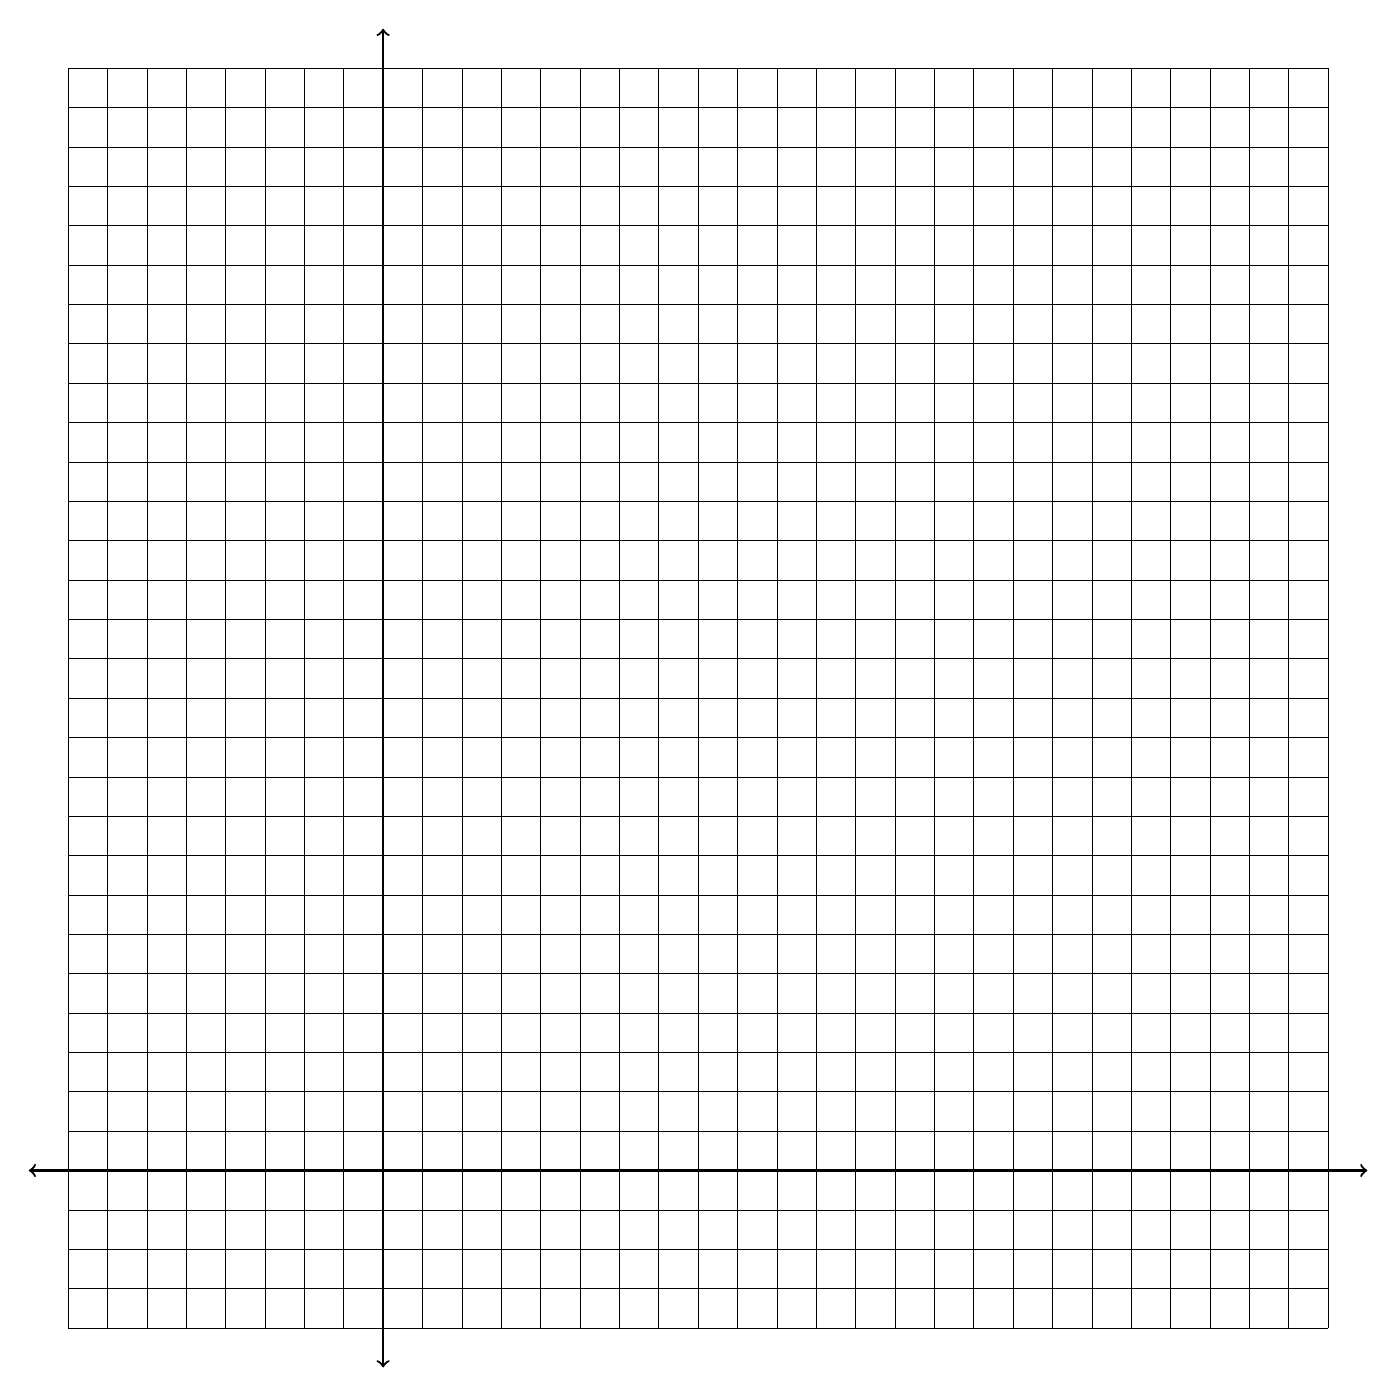
\begin{tikzpicture}
\draw[step=0.5,black,very thin] (0,0) grid (16, 16);
\draw[thick, <->] (-0.5, 2) -- (16.5, 2);
\draw[thick, <->] (4, -0.5) -- (4, 16.5);
\end{tikzpicture}
\end{center}


\pagebreak
\section*{Extension Problem}

Derive the quadratic equation. The term "Solving" a quadratic equation refers to solving an equation of the form
\begin{equation*}
ax^2 + bx + c = 0
\end{equation*}
This is equivalent to finding the points where the graph of $y = ax^2 + bx + c$ crosses the x-axis. Algebraically, this corresppnds to factorising the quadratic into factored form, in which case the null factor law provides the solutins. So for example, the solutions to the quadratic equation $2(x-3)(x+4) = 0$ are $x = 3$ and $x = -4$. As breifly mentioned earlier, not all quadratics can be factorised, and these quadratics correspond to those that do not cross the x-axis.

Sometimes factorisation can be difficult, but still possible, however. In these scenarios it can be useful to have a general formula for the solutions to a quadratic equation $ax^2 + bx + c = 0$, and luckily such a formula exists. Here the challenge is to derive that formula for yourself.

Hints:
\begin{itemize}
\item Begin by putting the general quadratic equation $ax^2 + bx + c = 0$ into vertex form by completing the square.
\item Once you have it in vertex form, try re-arranging the equation to get $x$ on it's own, i.e. something of the form $x = \hdots$.
\end{itemize}

\end{document}
